% Stage: — ／ 説明用コード: 概念は後で src/stages/01\_mpp/src/ftqc が実装
\chapter{エラー訂正符号とは}\label{ch:qec_codes}

\begin{chaptergoal}
  \begin{itemize}
  \item スタビライザ形式によって、符号空間・誤り・シンドロームを統一的に記述する方法を理解します。
  \item 論理演算子・符号距離・CSS 条件という、符号の性能と構造を表す語彙を身につけます。
  \item 表面符号（rotated surface code）の幾何と、$d=3$ の 9 データ量子ビット版を本書の主戦場として理解します。
  \item $[[15,1,3]]$ Reed–Muller 符号が魔法状態蒸留の土台になることの見通しを得ます。
  \end{itemize}
\end{chaptergoal}

第3章では、データ量子ビットを直接測定できず複製もできないという量子特有の制約から、アンシラを介した間接測定＝シンドローム測定が必然であることを確認しました。
3 ビット反復符号とパリティ検査 $Z_0Z_1$, $Z_1Z_2$ は、その考え方を最も小さな形で示した具体例にすぎません。
本章では、この具体例を一般化し、任意の量子誤り訂正符号を記述するための共通言語である\textbf{スタビライザ形式}を導入します。
そのうえで、符号の性能を表す\textbf{符号距離}、符号空間の内部で情報を運ぶ\textbf{論理演算子}、実装上扱いやすい構造を持つ\textbf{CSS 符号}という語彙を固定し、最終的に本書全体の主戦場となる\textbf{表面符号（rotated surface code）}の幾何、および魔法状態蒸留の土台となる$[[15,1,3]]$ Reed–Muller 符号への布石を与えます。
本章はあくまで語彙と定義を揃えることが目的であり、実際に Stim で符号を構築する手順（第7章以降、\codepath{src/stages/01_mpp/src/ftqc}）や復号アルゴリズム（第8章以降）には踏み込みません。

\section{スタビライザ形式}\label{sec:stabilizer}

\subsection{生成元}

$n$ 個の量子ビットに対するパウリ演算子（$I,X,Y,Z$ のテンソル積で位相 $\pm1,\pm\ii$ を許したもの）の全体をパウリ群 $\mathcal{P}_n$ と呼びます。
\textbf{スタビライザ符号}は、互いに可換で独立、かつ生成する群に $-I$ を含まない $n-k$ 個の Hermitian なパウリ演算子
\begin{equation}
  g_1, g_2, \dots, g_{n-k} \in \mathcal{P}_n, \qquad [g_i, g_j] = 0 \ (\forall i,j), \qquad -I \notin \langle g_1,\dots,g_{n-k}\rangle
\end{equation}
を\textbf{生成元}として指定し、これらが生成する可換な部分群
\begin{equation}
  \mathcal{S} = \langle g_1, \dots, g_{n-k} \rangle
\end{equation}
を\textbf{スタビライザ群}と呼びます\cite{gottesman1997stabilizer}。独立性は、どの生成元も残りの積で書けないことを意味し、これが符号空間の次元を $2^k$ と数えるために必要です。
第3章のパリティ検査 $Z_0Z_1$, $Z_1Z_2$ は、まさにこの $g_1,g_2$ に相当する生成元です。

\subsection{符号空間}

スタビライザ群のすべての元を固有値 $+1$ で満たす状態の集合を\textbf{符号空間}と呼びます。
\begin{equation}
  \mathcal{C} = \bigl\{\, \ket{\psi} \ :\ g_i \ket{\psi} = \ket{\psi}, \ \ i = 1,\dots,n-k \,\bigr\}
\end{equation}
生成元が互いに可換であることから、これらは同時固有状態を持ち、$\mathcal{C}$ は $2^k$ 次元の部分空間になります。
$k$ 個の\textbf{論理量子ビット}をこの部分空間に符号化し、残りの自由度（$n-k$ 個の生成元が担う分）を誤り検出に使う、というのがスタビライザ符号の基本構造です。
第3章の 3 ビット反復符号では $n=3$, $k=1$ で、$\ket{\psi_L}=\alpha\ket{000}+\beta\ket{111}$ が $Z_0Z_1=Z_1Z_2=+1$ を満たす符号空間そのものでした。

\subsection{誤りとシンドローム}

パウリ誤り $E \in \mathcal{P}_n$ が符号空間の状態 $\ket{\psi}\in\mathcal{C}$ に作用したとします。
各生成元 $g_i$ は $E$ と可換か反可換かのいずれかなので、
\begin{equation}
  g_i \, E \ket{\psi} = \pm E \, g_i \ket{\psi} = \pm E \ket{\psi}
\end{equation}
となります。
符号 $+$（可換）なら $g_i$ を測っても固有値は $+1$ のまま変化せず、符号 $-$（反可換）なら固有値は $-1$ に反転します。
この $n-k$ 個の固有値の組（あるいは $0/1$ に読み替えたビット列）を\textbf{シンドローム}と呼びます。

\begin{notebox}
  シンドロームは「$g_i$ と $E$ が可換か反可換か」だけを教え、$E$ そのものを特定するわけではありません。
  同じシンドロームを与える誤りは一般に複数存在し、それらの中からどの $E$ が起きたと\textbf{推定}するかを決める手続きが\textbf{復号}です。
  復号アルゴリズム（MWPM や BP+OSD など）は第8章以降で扱います。
\end{notebox}

これは第3章のパリティ検査を一般化した見方にほかなりません。
$X$ 誤りが 1 か所に起きると、隣接する $Z_0Z_1$ または $Z_1Z_2$ の固有値だけが反転し、その反転パターン（シンドローム）から誤りの位置を推定できる、というのが前章で確認した具体例でした。
一般のスタビライザ符号でも、誤りの検出と位置の推定はすべて「どの生成元が反転したか」という情報だけから行われます。

\section{符号距離・論理演算子・CSS 符号}\label{sec:css}

\subsection{論理演算子とノーマライザ}

符号空間 $\mathcal{C}$ の中で論理量子ビットに実際に作用する演算子を\textbf{論理演算子}と呼びます。
論理演算子は、符号空間を符号空間自身へ写す（$\mathcal{C}$ から出ない）必要があるので、すべての生成元と可換でなければなりません。
すべての生成元と可換なパウリ演算子の集合をパウリ群内の\textbf{中心化群} $C_{\mathcal P_n}(\mathcal{S})$ と呼びます。スタビライザ符号の文献では、パウリ群内のノーマライザ $N(\mathcal{S})=\{P\in\mathcal P_n:P\mathcal SP^\dagger=\mathcal S\}$ と同一視して $N(\mathcal S)$ と書くことが多く、本書もこの慣例を用います\cite{gottesman1997stabilizer}。
\begin{equation}
  \mathcal{S} \subset N(\mathcal{S}) \subset \mathcal{P}_n
\end{equation}
$\mathcal{S}$ 自身の元は符号空間に自明に（恒等的に）作用するので、実質的に意味のある論理演算子は商 $N(\mathcal{S})/\mathcal{S}$ の元、つまり「生成元とは可換だが、生成元の積そのものではない」パウリ演算子です。
1 個の論理量子ビットあたり 1 組の論理 $X_L$, $Z_L$ が存在し、これらは通常のパウリ演算子と同じ代数関係
\begin{equation}
  X_L Z_L = -Z_L X_L, \qquad X_L^2 = Z_L^2 = I
\end{equation}
を符号空間の上で満たします。
第3章の例では $X_L = X_0X_1X_2$、$Z_L = Z_0$（または $Z_1$, $Z_2$）が対応し、いずれも $Z_0Z_1$, $Z_1Z_2$ と可換ですが、生成元の積では表せません。

\subsection{符号距離}

論理演算子の中には、同じ論理作用を持ちながら重み（非自明なサイトの個数）が異なる複数の表現が存在します（$Z_L$ に生成元 $Z_0Z_1$ を掛けても論理作用は変わりません）。
\textbf{符号距離} $d$ は、$N(\mathcal{S})\setminus\mathcal{S}$ に属する演算子（＝非自明な論理演算子）の中で重みが最小のものの重みとして定義されます。
\begin{equation}
  d = \min_{\, P \,\in\, N(\mathcal{S}) \setminus \mathcal{S}} \operatorname{wt}(P)
\end{equation}
直感的には、$d$ は「シンドロームを変えずに論理情報を書き換えてしまう最小の誤りの個数（最小重み）」です。したがって重み $d-1$ 以下の Pauli 誤りは、シンドロームを生じるか、スタビライザとして符号空間に自明に作用します。後者は縮退符号では検出結果が変わりませんが、論理情報を損ないません。また訂正半径
\begin{equation}
  t = \left\lfloor \frac{d-1}{2} \right\rfloor
\end{equation}
とおくと、重み $t$ 以下の任意の Pauli 誤りに対して論理情報を回復できるという関係が従います。縮退符号では異なる物理誤りが同じ作用を持つため、実際の誤り自体が一意に特定されるという意味ではありません。
符号は 3 つの整数の組 $[[n,k,d]]$ で特徴づけられます：$n$ は物理量子ビット数、$k$ は論理量子ビット数、$d$ は符号距離です。
ただし、第3章の生成元 $\langle Z_0Z_1,Z_1Z_2\rangle$ は $Z_0$ という重み1の論理演算子を持つため、量子符号としては $[[3,1,1]]$ です。これは $X$ 誤りに対する距離 $d_X=3$ と $Z$ 誤りに対する距離 $d_Z=1$ を持つ、ビット反転だけを守る反復符号です。

\subsection{CSS 条件}

生成元を $X$ だけからなるものと $Z$ だけからなるものに完全に分離できるスタビライザ符号を\textbf{CSS 符号}（Calderbank–Shor–Steane 符号）と呼びます。
$X$ 型生成元の台（どの量子ビットに作用するか）を行に持つ行列を $H_X \in \mathbb{F}_2^{r_X \times n}$、$Z$ 型生成元の台を行に持つ行列を $H_Z \in \mathbb{F}_2^{r_Z \times n}$ とすると、$X$ 型どうし・$Z$ 型どうしは自動的に可換なので、可換性の条件は $X$ 型と $Z$ 型の間だけに残り、
\begin{equation}
  H_X H_Z^{\top} = 0 \pmod 2
\end{equation}
という\textbf{CSS 条件}に帰着します。
これは、$H_X$ を古典符号の検査行列とみなし、$H_Z$ をその双直交（あるいは双対に近い）別の古典符号の検査行列とみなすことに対応し、2 つの古典線形符号から 1 つの量子符号を組み立てる標準的な方法になっています。
論理量子ビット数は
\begin{equation}
  k = n - \operatorname{rank}(H_X) - \operatorname{rank}(H_Z)
\end{equation}
で与えられます。行の依存性は rank にすでに織り込まれています。論理 $X_L$ は $H_Z$ の核に属し $H_X$ の行空間に属さないベクトル、論理 $Z_L$ は逆に $H_X$ の核に属し $H_Z$ の行空間に属さないベクトルとして得られます\cite{calderbank1996css,steane1996qec}。

CSS 符号では $X$ 成分と $Z$ 成分のシンドロームを別々の古典検査行列で表せます。ただし $Y$ 誤りや相関ノイズは両成分を相関させるため、独立復号が常に最適とは限りません。次節の表面符号や本章末の $[[15,1,3]]$ 符号はいずれも CSS 符号です。
本書のシミュレータが Stim（スタビライザ回路専用）と Qulacs（非 Clifford 用状態ベクトル）を組み合わせるのも、Clifford 演算だけで閉じる部分を CSS のスタビライザ形式で高速に扱い、それだけでは扱えない非 Clifford な部分（第4節、第12章）を別の方法で扱うという分担に対応しています。

\section{表面符号（rotated surface code）}\label{sec:surface_code}

\subsection{データ配置とプラケット}

表面符号は、データ量子ビットを 2 次元格子上に配置し、隣接するデータ量子ビットの小さな集まり（\textbf{プラケット}）ごとに重み 4（境界では重み 2）の生成元を割り当てる CSS 符号です。
\textbf{rotated surface code}（回転表面符号）は、奇数距離の標準的な平面パッチでは $d \times d$ 個のデータ量子ビットを正方格子状に配置し、そのあいだの市松模様のプラケットに $X$ 型・$Z$ 型の生成元を交互に割り当てます。同じ距離の非回転パッチより少ないデータ量子ビット（この族では $n=d^2$）で実現できるため、実装上よく使われます\cite{fowler2012surface,dennis2002topological}。
図~\ref{fig:rotated_surface_d3} に、本書で主に使う $d=3$（$n=9$）の場合を示します。

\begin{figure}[htbp]
  \centering
  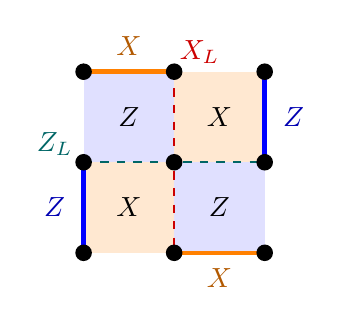
\begin{tikzpicture}[scale=1.15]
    % 上位に薄く各プラケットの塗りを置く
    \fill[blue!12] (0,1) rectangle (1,2);
    \fill[orange!18] (1,1) rectangle (2,2);
    \fill[orange!18] (0,0) rectangle (1,1);
    \fill[blue!12] (1,0) rectangle (2,1);
    % 境界の重み2生成元
    \draw[orange, ultra thick] (0,2) -- (1,2);
    \draw[orange, ultra thick] (1,0) -- (2,0);
    \draw[blue, ultra thick]   (0,1) -- (0,0);
    \draw[blue, ultra thick]   (2,2) -- (2,1);
    % 論理演算子（点線）
    \draw[red!80!black, thick, dashed]  (1,2) -- (1,1) -- (1,0);
    \draw[teal!80!black, thick, dashed] (0,1) -- (1,1) -- (2,1);
    % データ量子ビット
    \foreach \x in {0,1,2} {
      \foreach \y in {0,1,2} {
        \fill[black] (\x,\y) circle (2.6pt);
      }
    }
    % バルクプラケットのラベル
    \node at (0.5,1.5) {$Z$};
    \node at (1.5,1.5) {$X$};
    \node at (0.5,0.5) {$X$};
    \node at (1.5,0.5) {$Z$};
    % 境界プラケットのラベル
    \node[orange!70!black] at (0.5,2.28) {$X$};
    \node[orange!70!black] at (1.5,-0.28) {$X$};
    \node[blue!70!black]   at (-0.32,0.5) {$Z$};
    \node[blue!70!black]   at (2.32,1.5) {$Z$};
    % 論理演算子ラベル
    \node[red!80!black]  at (1.28,2.22) {$X_L$};
    \node[teal!80!black]  at (-0.32,1.2) {$Z_L$};
  \end{tikzpicture}
  \caption{$d=3$ の rotated surface code（9 データ量子ビット）。塗りと $X$/$Z$ の文字は生成元の型、太線は境界の重み 2 生成元、点線は論理演算子の代表元の一例を表します。}
  \label{fig:rotated_surface_d3}
\end{figure}

\subsection{境界と論理演算子}

図の中心にある 4 個の生成元は重み 4 で、市松模様のとおり $X$ 型と $Z$ 型が交互に配置されています。
格子の端では、はみ出す分のデータ量子ビットが存在しないため生成元の重みが 2 に落ち、これを\textbf{境界生成元}と呼びます。
rotated surface code には性質の異なる 2 種類の境界があります。

\begin{itemize}
  \item 境界の重み 2 生成元が $X$ 型になっている辺（図の上下）：これを \textbf{$X$ 境界}と呼びます。
  \item 境界の重み 2 生成元が $Z$ 型になっている辺（図の左右）：これを \textbf{$Z$ 境界}と呼びます。
\end{itemize}

本書の図と命名規約では、論理演算子をデータ量子ビットの鎖（同じ型のパウリ演算子を一列に並べた積）として実現し、\textbf{自分と同じ型と名付けた境界を結ぶ}代表元を選びます。rough/smooth や $X/Z$ 境界の呼称は文献の星・プラケット規約によって入れ替わり得るため、最終的な判定は名称ではなく、鎖が全スタビライザと可換で相補的な論理鎖と反可換かどうかで行います\cite{fowler2012surface}。
図では、$X_L$ が上下の $X$ 境界を結ぶ縦の鎖、$Z_L$ が左右の $Z$ 境界を結ぶ横の鎖として描かれています。
これは、同じ型のパウリ演算子どうしは常に可換なので、鎖が自分と同じ型の境界生成元とは自動的に可換になる（一方、反対の型の境界生成元とは、鎖がその境界を貫通しない限り可換にならない）という代数的な事情の帰結です。
図の $X_L$ と $Z_L$ はちょうど中央のデータ量子ビット 1 個だけを共有しており、この 1 点だけで反可換になることで、符号空間全体では正しく $X_LZ_L=-Z_LX_L$ が成り立ちます。

\subsection{$d=3$ という主戦場}

$d=3$ の rotated surface code は $[[9,1,3]]$ 符号で、生成元は重み 4 が 4 個、重み 2 が 4 個の合計 8 個です。
これは本書で繰り返し登場する最小構成であり、第7章以降で Stim を使って実際に構築し（\codepath{src/stages/01_mpp/src/ftqc} の幾何関数群）、第III部の格子手術や第12章の T ゲートに至るまで、一貫してこの $d=3$ パッチを土台にします。
$d$ を大きくすれば訂正能力（第3章で見た符号距離の効果）は上がりますが、量子ビット数は $n=d^2$ で増えるため、本書ではまず $d=3$ で語彙と手順を固め、必要な箇所でのみ距離を上げた場合の違いに触れる、という構成を取ります。

\begin{notebox}
  複数の $d=3$ パッチを隣接させ、境界どうしを一時的に結合・分離することで論理演算子どうしの合成測定を行う手法を\textbf{格子手術}と呼びます。
  境界の型（$X$ 境界か $Z$ 境界か）をどう合わせるかによって、測れる論理演算子の種類が決まります。
  幾何と生成元の組み合わせ規則の詳細は第10章（\codepath{src/stages/01_mpp/src/ftqc/geom_lattice_surgery.py} が対応）で扱い、本章では語彙の準備に留めます。
\end{notebox}

\section{魔法状態符号への布石（\texorpdfstring{$[[15,1,3]]$}{[[15,1,3]]}）}\label{sec:rm15}

\subsection{非 Clifford な資源の必要性}

表面符号のスタビライザ生成元は $X$ と $Z$ だけで書けるため、Hadamard・CNOT・$S$ ゲートといった Clifford 演算は、境界の操作や格子手術によって比較的単純に（多くの場合トランスバーサルに近い形で）実行できます。
しかし、Clifford 演算だけでは万能な量子計算はできません。
万能性のためには $T$ ゲート（あるいは Toffoli など）のような非 Clifford な演算が最低 1 種類必要です。

\begin{notebox}
  \textbf{Eastin--Knill の定理}：任意の単一物理サブシステムの誤りを検出できる有限次元の量子符号では、符号ブロック内の物理サブシステム同士を結合しない局所成分の積として作用するトランスバーサル論理ゲートだけで万能集合を構成できません。同じ物理ゲートを各サイトへかける場合だけに限らない定理です\cite{eastin2009transversal}。
  したがって、表面符号のようにトランスバーサルな Clifford 演算に適した符号だけでは $T$ ゲートを直接には実行できず、別の方法が必要になります。
\end{notebox}

その別の方法が\textbf{魔法状態}を用いたゲートテレポーテーションです。
あらかじめ $\ket{A} = T\ket{+}$ という特別な状態（魔法状態）を高い忠実度で用意しておけば、CNOT と測定、および測定結果に応じた $S$ 補正（既存の Clifford 演算だけ）を組み合わせることで、任意の論理量子ビットに $T$ ゲートを適用できます。
問題は、物理的に用意できる $\ket{A}$ には常に誤りが混じっており、そのままでは精度が不足することです。

\subsection{$[[15,1,3]]$ Reed–Muller 符号}

この精度不足を解決する標準的な方法が\textbf{魔法状態蒸留}です。
そこで使われる代表的な符号が、パラメータ $[[15,1,3]]$ の punctured quantum Reed--Muller CSS 符号で、古典 Reed--Muller 符号を土台に構成されます\cite{bravyi2005magic}。
$n=15$ 個の物理量子ビット、$k=1$ 個の論理量子ビット、符号距離 $d=3$ を持ち、$X$ 型・$Z$ 型それぞれの検査行列が古典 Reed–Muller 符号の生成行列・検査行列から具体的に書き下せる、という意味で表面符号と同じ CSS の枠組みに収まります。

この符号の重要な性質は、物理量子ビットへのトランスバーサルな $T$ または $T^\dagger$（論理演算の向きは符号・位相規約に依存）が論理 $T$ 型ゲートを実装することです（表面符号にはこの性質がなく、ここが両者の役割の違いです）。
この性質を利用して、15 個のノイズを含む $\ket{A}$状態を用意し、$[[15,1,3]]$ 符号の検査（シンドローム測定）を行い、シンドロームがすべて $0$ になった場合だけを採用する（\textbf{ポスト選択}する）ことで、出力される 1 個の $\ket{A}$ 状態の誤り率を、入力の誤り率 $p$ のおおむね 3 次
\begin{equation}
  p_{\mathrm{out}} \ \sim\ 35\, p^3
\end{equation}
まで抑制できます。ここで $35p^3$ は、独立同分布の入力 $Z$ 型魔法状態誤りを確率 $p$ で入れ、Clifford 操作と検査を理想化した模型の条件付き出力誤り率の先頭項です。距離が3という事実だけから係数35やこの確率式が決まるわけではありません\cite{bravyi2005magic}。
これを「15-to-1 蒸留」と呼びます。

\subsection{蒸留との接続}

本章で確認した通り、表面符号は Clifford 演算を効率よく実行するための符号であり、$[[15,1,3]]$ Reed–Muller 符号は非 Clifford な $T$ ゲートを実行するための資源（魔法状態）を高精度に用意するための、まったく別の符号です。
本書のハイブリッド構成（Stim によるスタビライザ回路のサンプリングと Qulacs による非 Clifford な状態ベクトル計算の併用）は、この 2 つの符号がそれぞれ担う役割の違いをそのまま反映しています。
$[[15,1,3]]$ 符号の検査行列の具体的な構成、蒸留のモンテカルロ検証、およびゲートテレポーテーション回路そのものは第12章（\codepath{src/stages/01_mpp/src/ftqc/t_gate.py} が対応）で扱い、本章ではその手前の語彙（$n,k,d$、CSS、トランスバーサル性）を確認するに留めます。

\section{まとめ}\label{ch4:summary}

\begin{itemize}
  \item スタビライザ形式は、互いに可換な生成元の集合 $\mathcal{S}$ によって符号空間を定義し、誤りとの可換・反可換関係からシンドロームを読み出す、量子誤り訂正符号の共通言語です。
  \item 論理演算子はノーマライザ $N(\mathcal{S})$ のうちスタビライザ群 $\mathcal{S}$ に属さない元であり、その最小重みが符号距離 $d$ を定めます。符号は $[[n,k,d]]$ の 3 つの整数で特徴づけられます。
  \item CSS 符号は生成元を $X$ 型と $Z$ 型に分離でき、可換性が $H_XH_Z^{\top}=0$ という古典的な条件に帰着します。シンドロームは成分別に表せますが、相関ノイズでは独立復号が最適とは限りません。
  \item rotated surface code は CSS 符号の具体例で、市松模様のプラケットと 2 種類の境界（$X$ 境界・$Z$ 境界）を持ち、論理演算子は同じ型の境界を結ぶ鎖として実現されます。$d=3$（$[[9,1,3]]$）が本書全体の主戦場です。
  \item スタビライザ操作だけでは万能計算にならず、Eastin--Knill の定理は単一符号のトランスバーサルゲートだけで万能集合を作れないことを述べます。$[[15,1,3]]$ Reed--Muller 符号による魔法状態蒸留は $T$ ゲート資源を供給します。
\end{itemize}

次章では、本章で固定した符号（特に表面符号）を時間軸に沿って動かし、符号サイクルの繰り返し、パウリフレーム追跡、Clifford と非 Clifford の切り分け、そして単体の符号だけでは扱えない場面（ストール）が統合シミュレータを必要とする理由を見ていきます。

\begin{exercise}
  \begin{enumerate}
    \item 3 ビット反復符号 $\mathcal{S}=\langle Z_0Z_1, Z_1Z_2\rangle$ について、$X_L=X_0X_1X_2$ がすべての生成元と可換であること、および $X_L$ が生成元の積では表せない（$\mathcal{S}$ に属さない）ことを確認しなさい。
    \item CSS 条件 $H_XH_Z^{\top}=0\pmod2$ が、$X$ 型生成元と $Z$ 型生成元の台の重なりが常に偶数個であることと同値であることを、$X$ と $Z$ の反交換関係から説明しなさい。
    \item 図~\ref{fig:rotated_surface_d3} の $d=3$ rotated surface code で、右下のデータ量子ビットに $Z$ 誤りが 1 個起きた場合、反転する生成元（シンドローム）はどれかを図から特定しなさい。また、その誤りが $X_L$ に何らかの影響を与えるかどうかを、$X_L$ と $Z$ の可換性から論じなさい。
    \item Eastin--Knill の定理が「単一のスタビライザ符号ではトランスバーサルな万能ゲート集合を持てない」と述べていることを踏まえ、表面符号と $[[15,1,3]]$ 符号という\textbf{2 つの符号}を併用する構成が、この定理をどのように回避しているかを 3 行程度で説明しなさい。
  \end{enumerate}
\end{exercise}
